%=== CHAPTER ONE (1) ===
%=== INTRODUCTION ===

\chapter{Introduction}
\begin{spacing}{1.5}
\setlength{\parskip}{0.3in}

The first chapter of the dissertation is almost invariably the Introduction. Generally, its purpose is to lead the readers into the problem you intend to attack in the project, to set the scene. The main points here consist of the background to the problem and your motivation in solving it. This then leads into the objectives and the scope of the project. It is good to conclude your Introduction with a section on the layout of the dissertation. It prepares the readers for what is to come

\section{Background}


Background goes here. Also you can put in some references~\cite{ronneberger2015unet}.

Here is a sample of table in \autoref{tabelsample}

\begin{table}[ht]
\centering
\caption{A table without vertical lines.}
\label{tabelsample}
\begin{tabular}[t]{lcc}
\hline
&Treatment A&Treatment B\\
\hline
John Smith&1&2\\
Jane Doe&--&3\\
Mary Johnson&4&5\\
\hline
\end{tabular}
\end{table}%

Also can try to refer to this image in \autoref{fig:boundingboxexample}.


\begin{figure}[ht]
\centering
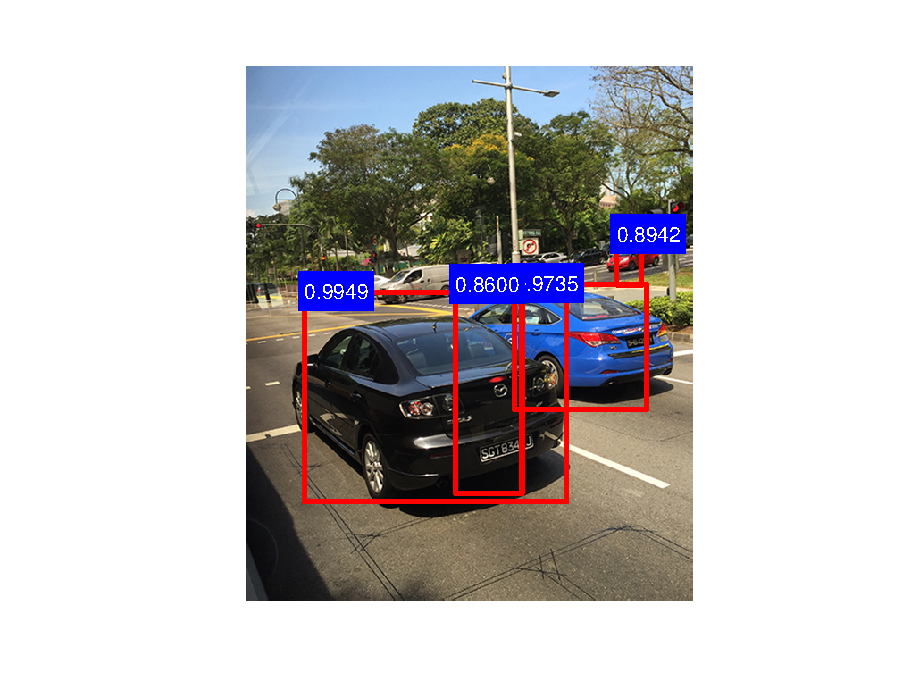
\includegraphics[width=4in, fbox]{Chapter1/boundingbox.eps}
\caption{Bounding-box example of cars.}
\label{fig:boundingboxexample} 
\end{figure}


\section{Motivation}


\section{Objectives and Specifications}



\section{Major contribution of the Dissertation}



\section{Organisation of the Dissertation}


\end{spacing}
%=== END OF CHAPTER ONE ===
\newpage


